\documentclass[11pt,a4paper,twoside]{article}
\usepackage{tascar}
\pagenumbering{arabic}
\pagestyle{empty}
\showtutorialtrue
\begin{document}
\setcounter{tutorial}{6}
\begin{tutorial}{\tascar{} on stage: Music and light processing}{GLPO}
Tips and tricks for processing of music. You will create a virtual
live mix of a jazz band, and can compare it to a conventional stereo
mixing approach. Add motion to your virtual stage, add light to your
show. Try ambisonic dance-floor mixing.

\begin{learnitems}
\item Mixing, direct-to-reverb ratio, source width control
\item Parametric motion control
\item All the other things \tascar{} can do
\end{learnitems}

\begin{appitems}
\item Creative / art / music projects
\item Parties in the NeSSy foyer
\item Experiments in the Gesture lab
\end{appitems}

\medskip

\centerline{
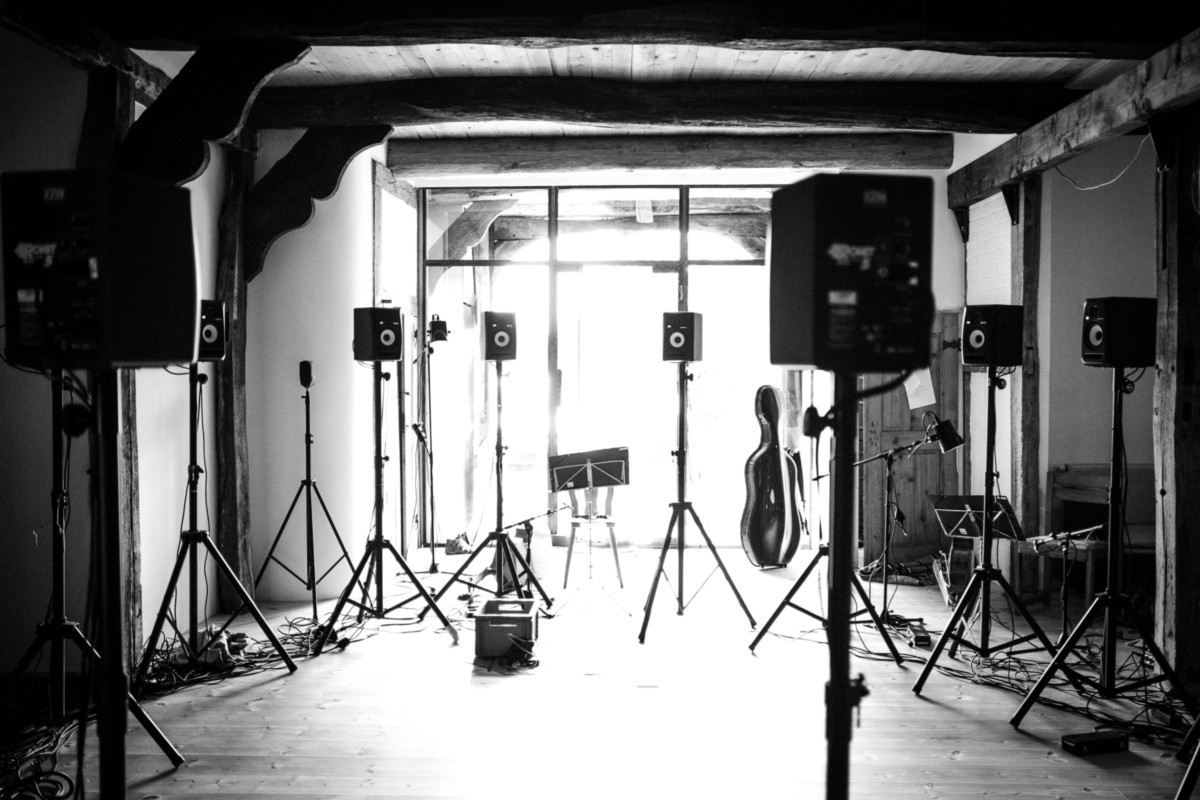
\includegraphics[width=0.45\columnwidth]{tascaronstage1.jpg}
\hskip8mm
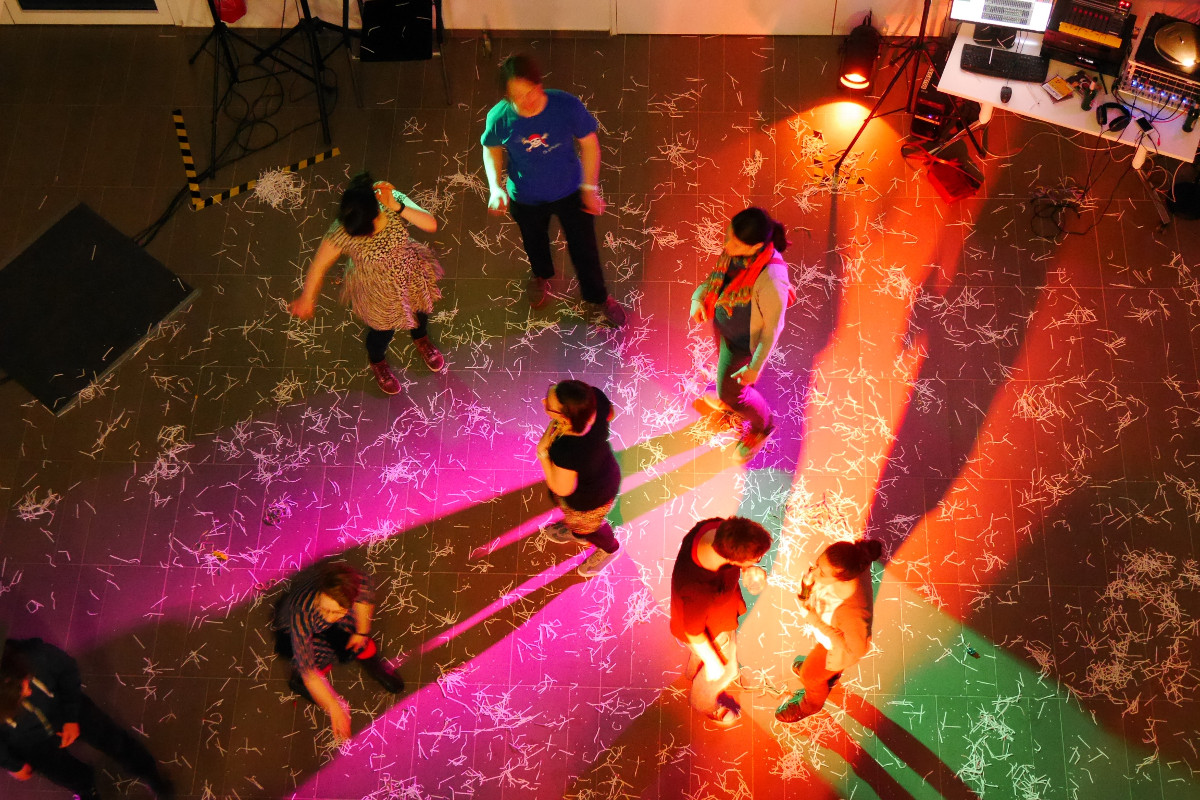
\includegraphics[width=0.45\columnwidth]{tascaronstage2.jpg}
}
\end{tutorial}

\ifshowtutorial

\newpage

\subsection*{Part 1: Mixing music}

We prepared an Ardour (\url{http://ardour.org}) session with a
recording of a jazz ensemble
(\url{http://lalists.stanford.edu/lau/2011/05/0534.html}).
%
First try to create a stereo mix (two loudspeakers are already connected).
%
Use gain and panning. If you add audio plugins, make sure to add them pre-fader (you will see later why).
%
Save your session before adding plugins! Evil plugins (there are some
out in the open source world) may crash your audio workstation.

Are you happy with the result?
%
Now leave the session Ardour open, but press the mute button on the master fader.
%
Open the ``tutorial7.tsc'' TASCAR session file. This will create a
TASCAR session with the instruments, connected to the Ardour tracks.
%
How does it work?
%
In each track you may find a ``send''. Each send creates a jack output
port. Each Ardour ``send'' audio port is connected to the
corresponding sound vertex in TASCAR.

Now place the band on the stage. The drum set, guitar and bass have
more than one sound vertex -- try to distribute them in space. If you
configure the vertical position of the sound vertices, all objects can
remain on the floor (or stage) level.

\begin{lstinputlisting}[language=tsc,caption={},linerange=10-11,firstnumber=10]{../examples/tutorial7_music_light/tutorial7.tsc}
\end{lstinputlisting}

Now all instruments are still in the origin. You can edit the
instrument positions in the TASCAR file by adding a position to each
object, as it was already done for the receiver:
\begin{lstinputlisting}[language=tsc,linerange=30-32,firstnumber=30,caption={}]{../examples/tutorial7_music_light/tutorial7.tsc}
\end{lstinputlisting}
Press the ``reload'' button after each change. Tired of all the manual
changes? Use our GNU Octave positioning tool \verb!jazzpos.m!. This
will send positions via OSC. But note: These are not saved in the
session file; you have to manually edit the positions once you are
happy.

Source width: An instrument is usually not a point source. Increase the size of an instrument, e.g., by using the system command \verb!send_osc!:
\begin{verbatim}
 send_osc 9877 /scene/Keyboards/*/size 1
\end{verbatim}
You can isolate (``solo'') sounds by pressing the ``S'' button for the desired sounds and receiver pair.

Need some room? Add a room acoustic model of Wilhelm13
(\url{http://www.wilhelm13.de}) -- un-comment the \verb!facegroup! elements:
\begin{lstinputlisting}[language=tsc,linerange=35-37,firstnumber=35,caption={}]{../examples/tutorial7_music_light/tutorial7.tsc}
\end{lstinputlisting}
This will add early reflections (second order geometric image source
model). To add also diffuse reverberation, you may use an impulse
response recorded in the foyer of the house of hearing:
\begin{lstinputlisting}[language=tsc,linerange=40-40,firstnumber=40,caption={}]{../examples/tutorial7_music_light/tutorial7.tsc}
\end{lstinputlisting}
\begin{lstinputlisting}[language=tsc,linerange=44-55,firstnumber=44,caption={}]{../examples/tutorial7_music_light/tutorial7.tsc}
\end{lstinputlisting}

Do you like your TASCAR mix? Compare the results to your stereo mix! (mute receivers in TASCAR, un-mute master fader in Ardour).

\subsection*{Part 2: Light control with TASCAR}

TASCAR can control light. We use the DMX512 standard for controlling
lights (\url{https://en.wikipedia.org/wiki/DMX512}). TASCAR provides
drivers for the network-based Artnet protocol (used in the Gesture
lab) and for the openDMX USB device by Entec (used in this
tutorial). The tools are documented in the TASCAR manual, section
6.16.

In TASCAR, a light scene can be used to create static or moving light
settings. To track objects, first create a audio scene (see \verb!tutorial7light.tsc!):
\begin{lstinputlisting}[language=tsc,linerange=4-16,firstnumber=4,caption={}]{../examples/tutorial7_music_light/tutorial7light.tsc}
\end{lstinputlisting}
Now you can setup the lightscene to track objects in the audio scene:
\begin{lstinputlisting}[language=tsc,linerange=19-19,firstnumber=19,caption={}]{../examples/tutorial7_music_light/tutorial7light.tsc}
\end{lstinputlisting}
Try to setup a second moving source, and track a second light object
with a different color (hint: use \verb!objects="/*/src*"!).

Now try to control the lights via OSC. For this, check the list of OSC
variables, then open a terminal, and use the command \verb!send_osc!
to send the colors.
\fi
\end{document}
%%  LocalWords:  TASCAR Ardour tsc OSC
